
\chapter{启动}
\label{chap:booting}

好的,我们已经在系统上安装了Slackware,现在我们要学的不是别的,就是控制
你机器启动顺序的东西,以及防止有一天不能用了,还要学习如何修复它。如果
你用Linux的时间够长,范个错误导致不能启动是尽早的事。幸运的是,不需要重
装系统我们就能修复它。许多操作系统都隐藏底层如何工作的细节,与之相反,
Linux(这里尤指Slackware)让我们能完全控制启动过程。只要简单地修改一两
个配置文件,重新运行引导装载程序的安装程序,就是简单快速地对系统进行修
改(或者破坏)。Slackware甚至使得多操作系统启动变得很容易,如和其它的
Linux发行版或Microsoft Windows一起启动。

\section{mkinitrd}
\label{sec:booting:mkinitrd}

进行其它步骤之前,快速地讨论一下Linux内核是有必要的。Slackware Linux包
括了至少两个,有时更多的不同内核。它们都是从相同的源码编译而来,也因此
是``一致''的,但它们不是一模一样的。根据你的系统架构及Slackware的版本,
安装器可能已经用一好几个内核来引导你的系统。一些内核是为单处理处系统准
备的,另一些是为多处理器系统准备的(在32位的Slackware中)。在古老的年
代,有许许多多用于安装在不同磁盘控制器下的内核。对于我们的讨论,重要的
是``huge''内核和``generic''内核。

如果你查看你的\path{/boot}文件夹,你会看到你的系统里安装了好几个内核。
\begin{Verbatim}[frame=single,commandchars=\\\{\}]
darkstar:~# \textbf{ls -1 /boot/vmlinuz*}
/boot/vmlinuz-huge-2.6.29.4
/boot/vmlinuz-generic-2.6.29.4
\end{Verbatim}
这里,可以看到,我安装了两个内核,\path{vmlinuz-huge-2.6.29.4}及
\path{vmlinuz-generic-2.6.29.4}。Slackware的每个发行版都包含了好几个
不同内核版本,有时甚至取了不同的名字,所以如果在你的机子上看到的内容跟
我不同,不要担心。

Huge内核就像你感觉的一样,很大。然而,这并不意味着这个内核里包含了所有
能有的驱动,也不意味着所有的驱动都编译到了内核中。相反,这些内核是为了
从Slackware支持的每种你能想到的电脑(当然,也有一些电脑不能通过它们启
动)启动而编译的。这些内核理所当然地含有一些支持你的机器没有的(也可能
永远不会有的)硬件的驱动,但这并没有关系。Slackware包含这些内核是有道
理的,其中最重要的一条就是Slackware的安装器要用到它——Slackware的安装盘
就是在这上面运行的。如果你是让安装器自动选择内核进行启动的话,很有可能
选择的就是这些内核,主要原因就是它们支持很多的硬件。相反,不使用外部模
块的放,generic内核支持的硬件就很少。如果你想用generic内核的话,你就必
须用到叫作initrd的东西,它是用mkinitrd(8)这个工具做的。

那么,为什么还会有generic内核呢?当前,Slackware开发团队有一些推荐使用
generic 内核的理由。最明显的一个就是大小。在解压、载入内存之前,huge内
核的大小的几乎是generic内核的两倍。如果你是在一台很老的机子上运行,拥
有的内存很小的话,那么generic节省的空间还是很可观的。与之不同的是,我
们的理由考虑的是质量问题。huge内核中的驱动会时不时地冲突,而且一般来说,
huge内核的表现不如generic内核。并且,使用generic内核的话,我们可以单独
地为特定驱动指定一些特别的参数,而不是必须通过内核命令行来传递。比起将
驱动编译进内核,Slackware中的一些工具,在驱动编译成模块的情况下运行得
更好。如果还是不好理解的话,只要想着``huge内核=好,generic内核=更好''。

不幸的是,generic用起来不像huge内核那样直接。要使用generic内核启动系统,
你还必须使用一个包含基本模块的initrd。所谓的模块,是指从内核源码编译而
得的一些部件,这些部件在内核运行时能动态地加载或卸载(使用modprobe(8)是
一个理想的选择)。以增加一点复杂性为代价,这种方法使系统更为灵活。你可
以把模块看作是设备驱动。至少在本节里能这么干。一个典型的例子是,无论你
的root分区用的是什么文件系统\footnote{如ext2,ext3,ext4,xfs等。译者注。},你都要
加入支持相应文件系统的模块。如果你的分区是在一块SCSI或RAID硬盘上,你还
要加入支持它们模块。最后,如果你用到软件模拟的RAID、磁盘加密或LVM,那
么不管你用不用generic内核,都要创建一个initrd。

所谓的initrd,是一个压缩的cpio(1)归档文件。所以要创建的话不是很直接。
庆幸吧,Slackware已经包含了能容易创建它的工具——mkinitrd。对它的全面讨
论已经超出了本书的范围,但我们会讨论一些重点概念。想看完整的解释,要么
去看它的man手册,要么运行带参数[\verb|--|help]的mkinitrd。
\begin{Verbatim}[frame=single,commandchars=\\\{\}]
darkstar:~# \textbf{mkinitrd --help}
mkinitrd creates an initial ramdisk (actually an initramfs cpio+gzip
archive) used to load kernel modules that are needed to mount the
root filesystem, or other modules that might be needed before the
root filesystem is available.  Other binaries may be added to the
initrd, and the script is easy to modify.  Be creative.  :-)
.... many more lines deleted ....
\end{Verbatim}
使用mkinitrd的时候,你必须了解一些信息:你的root分区、root文件系统、你
用到的硬盘控制器\footnote{简单的理解就是硬盘类型,如PATA、SATA等。译者
注。}以及你是否用到了LVM、软件RAID或磁盘加密。如果你正在使用某些SCSI控
制器(并且root分区就放在这个控制器上),那么你只要知道root文件系统及分
区类型。假设你是用huge内核启动进入Slackware安装界面的,那么你可以很容
易地用mount命令来找到这些信息,当然,也可以通过查看
\path{/proc/mounts}中的内容得到。
\begin{Verbatim}[frame=single,commandchars=\\\{\}]
darkstar:~# \textbf{mount}
/dev/sda1 on / type ext4 (rw,barrier=1,data=ordered)
proc on /proc type proc (rw)
sysfs on /sys type sysfs (rw)
usbfs on /proc/bus/usb type usbfs (rw)
/dev/sda2 on /home type jfs (rw)
tmpfs on /dev/shm type tmpfs (rw)
\end{Verbatim}
在上面这个例子中,可以看到,root分区位于\path{/dev/sda1}中,类型是
ext4。如果想为这个系统创建一个initrd,我们就可以告诉initrd这些信息。
\begin{Verbatim}[frame=single,commandchars=\\\{\}]
darkstar:~# \textbf{mkinitrd -f ext4 -r /dev/sda1}
\end{Verbatim}
大多数情况下,mkinitrd能自动检测到这些信息,但手动指定这些信息也不会让
你少块肉。现在我们创建了我们自己的initrd,接下来只要告诉LILO去哪找到这
个文件就行了。我们会在下一节中集中介绍这个内容。

然而,如果去查看mkinitrd的所有不同选项是很痛苦的,如果想记住它们就更糟
糕了,尤其是在你想一口气试用我们不同的内核。对于Slackware开发团队而言
这是很无趣但又痛苦的事,所以他们想到编写一个简单的配置文件:
\path{mkinitrd.conf(5)}。在\path{/etcmkinitrd.conf.sample}文件夹下
可以找到一个文件,使用这个文件就可以为很容易地为我们的系统做配置。下面
晒晒我的。
\begin{Verbatim}[frame=single,commandchars=\\\{\}]
darkstar:~# >/prompt>\textbf{cat /etc/mkinitrd.conf.sample}
# See "man mkinitrd.conf" for details on the syntax of this file
#
SOURCE_TREE="/boot/initrd-tree"
CLEAR_TREE="0"
OUTPUT_IMAGE="/boot/initrd.gz"
KERNEL_VERSION="\$(uname -r)"
#KEYMAP="us"
MODULE_LIST="ext3:ext4:jfs"
#LUKSDEV="/dev/hda1"
ROOTDEV="/dev/sda1
ROOTFS="ext4"
#RESUMEDEV="/dev/hda2"
#RAID="0"
LVM="1"
#WAIT="1"
\end{Verbatim}
至于每行都有什么作用,并自行查看 \textbf{mkinitrd.conf} 的man手册。将
该样例文件复制到\textbf{/etc/mkinitrd.conf}并作出合适的修改。一旦进行
了正确的设置,我们只需要以参数[-F]运行mkinitrd即可。无需记住这些晦涩的
参数,mkinitrd就会自动创建一个正确的initrd文件,并且自动安装。

如果你不确定在配置文件或命令行中应指定什么样的选项,还有一个终级的必杀。
Slackware 中有一个帅气的工具,能告诉我们用现在运行的内核,创建一个
initrd要使用什么参数,这个工具是
\path{/usr/share/mkinitrd/mkinitrd\_command\_generator.sh}。运行这个脚
本,它就会生成一个适用于现在操作系统的mkinitrd的参数,但你最好还是检查
一遍。
\begin{Verbatim}[frame=single, commandchars=\\\{\}]
darkstar:~# \textbf{/usr/share/mkinitrd/mkinitrd\_command\_generator.sh}
mkinitrd -c -k 2.6.33.4 -f ext3 -r /dev/sda3 -m \textbackslash{}
  usbhid:ehci-hcd:uhci-hcd:ext3 -o /boot/initrd.gz
\end{Verbatim}

\section{LILO}
\label{sec:booting:lilo}

LILO是Linux Loader的缩写,是Slackware Linux的默认引导装载程序。如果你
用过其它版本的话,你可能对GRUB更熟悉。如果你更喜欢GRUB的话,可以在
Slackware的CD上找到\texttt{extra/}文件夹,GRUB的安装包就在里面。由于
LILO是Slackware默认的引导装载程序,我们只对LILO进行讨论。

LILO的设置比较麻烦,可能会吓到一些新手,所以Slackware自带了一个特殊的
设置程序,叫作liloconfig。一般情况下,第一次运行liloconfig的是
Slackware安装器,但你也可以自己在终端中运行。

\begin{figure}[htpb]
  \centering
  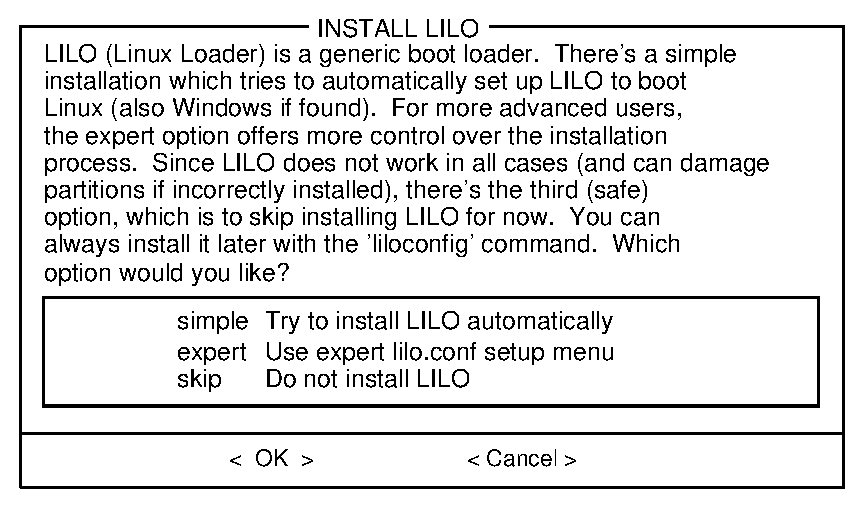
\includegraphics[width=0.8\textwidth]{images/installation/setup-lilo.eps}
  \caption{liloconfig}
  \label{fig:booting:setup-lilo}
\end{figure}

运行liloconfig有两个模式:简单级和专家级。``简单级''可以自动为你完成设
置。如果Slackware是你机子上唯一的系统,那么使用``简单级''就可以了,通
常情况下它都能快速准确地完成任务。同时,它还擅长于检测机子上安装的
Windows,并将它的启动项加入\path{/etc/lilo.conf},那么在启动的时候,
你就能选择启动哪个系统了。

要使用``专家级''的话,你就要对Slackware的root分区有所了解。如果知道其
它Linux系统的root分区在哪的话,你也可以添加它们的启动项,但这个过程并
不像你想像中的那样。liloconfig会尝试使用Slackware的内核来启动每个Linux
系统,而这大概不是你想要的行为。庆幸的是,专家级中对Windows分区的设置
是一致的。使用专家级的一个提示:记得把LILO装到主引导记录(MBR)中。我
们曾建议把引导装载程序装到root分区中并将该分区设置为可引导的。现在,
LILO已经足够成熟,装到MBR上也是很安全的。事实上,安装到MBR上反而更不会
遇到问题。

liloconfig对于快速设置引导装载程序而言是绝佳的选择,但如果你想了解它的
原理,那么你应该查看LILO的配置文件:位于\texttt{/etc}下的
\texttt{lilo.conf(5)}。\path{/etc/lilo.conf}被分为几个部分。在顶部,
能看见一个``全局''的部分,在这里可以指定LILO安装的位置(一般是MBR)、
启动时要显示的图像或屏幕的设置,以及LILO启动默认项的等待时间。下面是我
的lilo.conf文件的全局部分,为了显示已经分成不同的部分。

\begin{Verbatim}[frame=single, commandchars=\\\{\}, numbers=left, numberblanklines=fasle]
# LILO configuration file

boot = /dev/sda
  bitmap = /boot/slack.bmp
  bmp-colors = 255,0,255,0,255,0
  bmp-table = 60,6,1,16
  bmp-timer = 65,27,0,255

append=" vt.default_utf8=0"
prompt
timeout = 50

# VESA framebuffer console @ 1024x768x256
vga = 773
.... many more lines ommitted ....
\end{Verbatim}
想了解LILO的所有选项,你可以查看\texttt{lilo.conf}的man手册。我们在本
文档中只讨论最常见的选项。

第一件要注意的事是"boot"行。该行决定了LILO将要安装到什么位置。要将它安
装到硬盘的主引导记录(MBR)中,只要在该行填上硬盘的设备条目。本例中,
我用的是SATA硬盘,但是以一个SCSI设备名字显示的,即\path{/dev/sda}。
要将LILO安装到一个分区的引导块中,就要在该行填上该分区的设备条目。例如,
如果你要安装到你电脑中唯一的SATA硬盘中的第一个分区,相应的设备条目为
\path{/dev/sda1}。

``prompt''选项只是为了告诉LILO,给出一个提示,让你选择要启动的系统。要启
动的系统在文件的后面会列出,一个系统占一个段。我们过一会再说明。
``timeout''选项告诉LILO在启动默认OS之前,应该等待多长时间(以十分之一秒
计算)。我的例子中,等待时间为5秒。有些系统要花很长的时间才能显示启动
屏幕,所以你应该设置比我更长的等待时间。这就是为什么简单级的LILO安装设
置了一很长的等待时间(大概是整整两分钟)。``append''行是由liloconfig设置
的。你在查看(最好看一下)你自己的\path{/etc/lilo.conf}时,应该能看
到类似的东西。对这行我们不深入讨论,所以你只要相信存在即合理。

我们已经浏览了全局部分,现在应该看看操作系统部分。每个Linux操作系统段
都以一个``image''行开始。Microsoft Windows操作系统用一个``other''行来指定。
让我们看看一个即有Slackware也有Microsoft Windows的
\path{/etc/lilo.conf}的样本吧。

\begin{Verbatim}[frame=single, commandchars=\\\{\}, numbers=left, numberblanklines=fasle]
# LILO configuration file
... global section ommitted ....
# Linux bootable partition config begins
image = /boot/vmlinuz-generic-2.6.29.4
  root = /dev/sda1
  initrd = /boot/initrd.gz
  label = Slackware64
  read-only
# Linux bootable partition config ends
# Windows bootable partition config begins
other = /dev/sda3
  label = Windows
  table = /dev/sda
# Windows bootable partition config ends
\end{Verbatim}
对于像Slackware的Linux操作系统,``image''行用于指定采用哪个内核启动。本
例中,我们使用\path{/boot/vmlinuz-generic-2.6.29.4}这个内核。剩下的
段看看字面就知道意思了。它们告诉LILO从哪去找root文件系统,用哪个(如果有
的话)initrd,以及开始挂载root文件系统时用只读权限。``initrd''行对于用
generic内核的用户,或是用到LVM或软件RAID的用户而言是十分重要的。因为它
告诉LILO(及内核)在哪可以找到用mkinitrd生成的initrd文件。

一旦设置好了\path{/etc/lilo.conf},只要运行lilo(8)就可以安装了。不像
GRUB及其它的引导装载程序,只要对配置文件作了改变,LILO就要求重新执行
lilo命令,否则新的(改变后的)引导装载程序镜像是不会安装的,也因此所做
的修改不会得以表现。


\begin{Verbatim}[frame=single, commandchars=\\\{\}]
darkstar:~# \textbf{lilo}
Warning: LBA32 addressing assumed
Added Slackware *
Added Backup
6 warnings were issued.
\end{Verbatim}

在执行lilo时你会看到很多警告信息,不要害怕。只要看到的不是一个致命错误
(fatal error),那都没事。特别的,如果看到一个LBA32地址警告是很正常的。

%TODO: dule boot

%%% Local Variables: 
%%% mode: latex
%%% TeX-master: "../SlackGuide"
%%% End: 
